\section{Transformations}
\greenbf{Linear functions:}
$f(ax + by) = af(x) + bf(y)$

\greenbf{Homogeneous Coordinates:} Raise dimensionality by 1 and set its coordinate to 1. 
\begin{center}
$
\begin{pmatrix}
    %\begin{smallmatrix} 
        x & y 
    %\end{smallmatrix} 
\end{pmatrix}^T \leftrightarrow 
\begin{pmatrix}
    %\begin{smallmatrix} 
        xw & yw & w 
    %\end{smallmatrix} 
\end{pmatrix}^T
w \in \mathbb{R}\backslash\{0\}
$
\end{center}
This allows non-linear transformations to still be denoted as matrices. \\
\greenbf{Translation:}
    $\begin{bmatrix}
        %\begin{smallmatrix}
            1 & 0 & t_x \\
            0 & 1 & t_y \\
            0 & 0 & 1
        %\end{smallmatrix}
    \end{bmatrix}$
\greenbf{Scale:}
$\begin{bmatrix}
    %\begin{smallmatrix}
        s_x & 0 & 0 \\
        0 & s_y & 0 \\
        0 & 0 & 1
    %\end{smallmatrix}
\end{bmatrix}$ \\
\greenbf{Rotations:}
Not commutative. $R^{-1} = R^T$. \\
3D-rotate(x):
$\begin{bmatrix}
    %\begin{smallmatrix}
        1 & 0 & 0 & 0 \\
        0 & cos(\theta) & -sin(\theta) & 0 \\
        0 & sin(\theta) & cos(\theta) & 0\\
        0 & 0 & 0 & 1
    %\end{smallmatrix}
\end{bmatrix}$\\
3D-rotate(y):
$\begin{bmatrix}
    %\begin{smallmatrix}
        cos(\theta) & 0 & sin(\theta) & 0 \\
        0 & 1 & 0 & 0 \\
        -sin(\theta) & 0 & cos(\theta) & 0\\
        0 & 0 & 0 & 1
    %\end{smallmatrix}
\end{bmatrix}$\\
3D-rotate(z):
$\begin{bmatrix}
    %\begin{smallmatrix}
        cos(\theta) & -sin(\theta) & 0 & 0 \\
        sin(\theta) & cos(\theta) & 0 & 0 \\
        0 & 0 & 1 & 0\\
        0 & 0 & 0 & 1
    %\end{smallmatrix}
\end{bmatrix}$\\
To rotate around arbitrary axes, see Quaternions. 

\greenbf{Shear:}\\
$
\begin{bmatrix}
    %\begin{smallmatrix}
    1 & 0 & sh_x & 0 \\
    0 & 1 & sh_y & 0 \\
    0 & 0 & 1 & 0 \\
    0 & 0 & 0 & 1
    %\end{smallmatrix}
\end{bmatrix}
$$
\begin{bmatrix}
    %\begin{smallmatrix}
    1 & sh_x & 0 & 0 \\
    0 & 1 & 0 & 0 \\
    0 & sh_z & 1 & 0 \\
    0 & 0 & 0 & 1
    %\end{smallmatrix}
\end{bmatrix}
$$
\begin{bmatrix}
    %\begin{smallmatrix}
    1 & 0 & 0 & 0 \\
    sh_y & 1 & 0 & 0 \\
    sh_z & 0 & 1 & 0 \\
    0 & 0 & 0 & 1
    %\end{smallmatrix}
\end{bmatrix}
$\\
\greenbf{Rigid Transformation:} 
Transformation that preserves vector length. (Only rotation \& translation)

\greenbf{Change Coordinate Systems: }

$p' = \begin{bmatrix}
    \mathbf{r_1} & \mathbf{r_2} & \mathbf{r_3} & \mathbf{t} \\
    0 & 0 & 0 & 1
\end{bmatrix}p$ where $\mathbf{r_1},\mathbf{r_2},\mathbf{r_3}$ are the old axes in the new system and $\mathbf{t}$ is the translation from new origin to old origin. \\
Transform normals with:\\
$p' = Mp \Rightarrow n' = (M^{-1})^Tn$

\subsection*{Quaternions}
Rotations and translations efficiently. 
\begin{center}
   $z = a + bi + cj + dk$\\
    $\begin{pmatrix}
    u & v & w
    \end{pmatrix}^T \leftrightarrow 0 + ui + vj + wk$
\end{center}
\greenbf{Properties:}
$i^2 = j^2 = k^2 = -1 \quad ijk = -1 \\ ij = k \quad ki = j \quad jk = i \\ ji = -k \quad ik = -j \quad kj = -i$\\
\greenbf{Vector form:} $z = s + \mathbf{v} \quad$ \textbf{v} is a vector, s is a scalar\\
\greenbf{Product:} $(s_1 + v_1) \cdot (s_2 + v_2) = s_1s_2 - v_1 \cdot v_2 + s_1v_2 + s_2v_1 + v_1 \times v_2$\\
\greenbf{Conjugate:} $\overline{(s_1 + v_1)} = s_1 - v_1, \quad z\overline{z} = \lVert z \rVert ^2 $\\
\greenbf{Inverse:} $z^{-1} = \frac{\overline{z}}{\lVert z \rVert ^2}, \quad 1 = z^{-1}z = zz^{-1} $\\
\greenbf{Rotation:} Vector $a = (x, y, z)^T$, rotate around $u$
\begin{compactenum}
    \item $(x,y,z)^T \rightarrow $ Quaternion $p = 0 + xi + yj + zk$
    \item Compute $q = cos(\frac{\theta}{2}) + sin(\frac{\theta}{2})\frac{u}{\lVert u \rVert}$ and $q^{-1} = \overline{q}$
    \item $p' = qpq^{-1}$
\end{compactenum}

\subsection*{Projections}
\greenbf{Perspective Projection:}\\
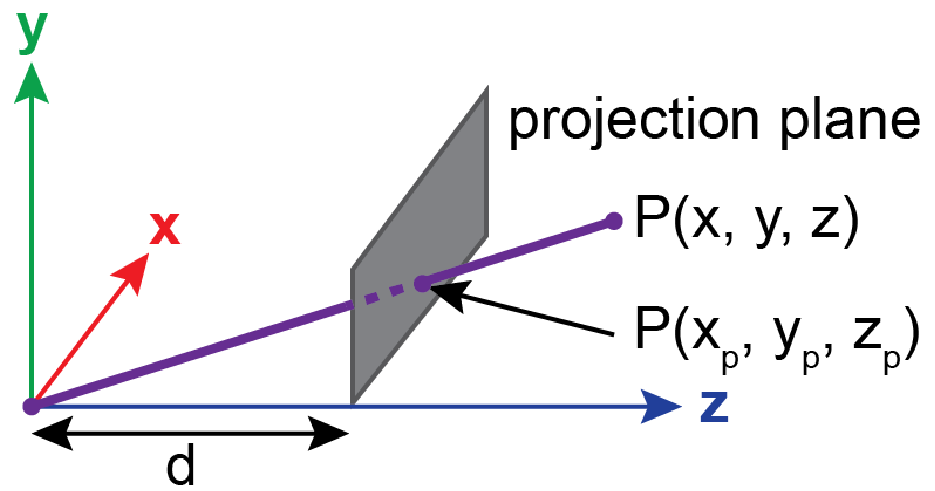
\includegraphics[width = 0.6\columnwidth]{assets/arjun/perspective projection.png}\\
You can imagine the projection plane to be the screen space and the origin the camera.\\
$x_p = dx/z \quad y_p = dy/z \quad z = d$

$ M_{per} = 
\begin{bmatrix}
    %\begin{smallmatrix}
        1 & 0 & 0 & 0\\
        0 & 1 & 0 & 0\\
        0 & 0 & 1 & 0\\
        0 & 0 & 1/d & 0
    %\end{smallmatrix}
\end{bmatrix}$\\
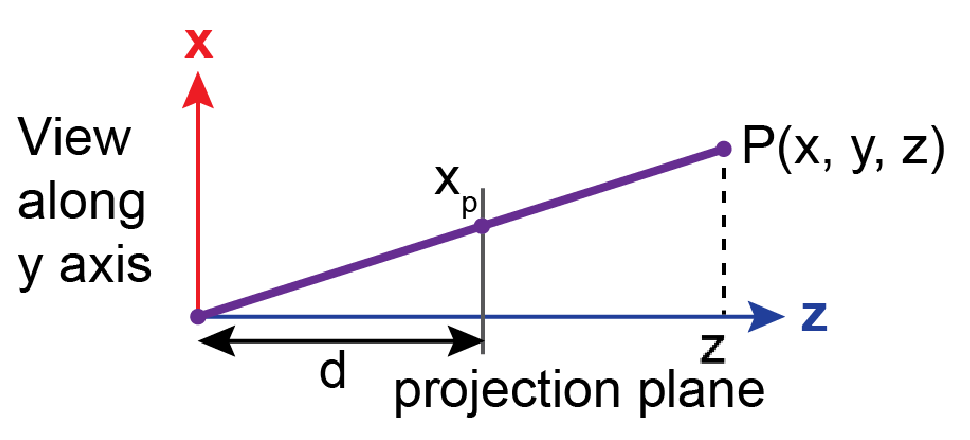
\includegraphics[width = 0.6\columnwidth]{assets/arjun/perspective projection y axis.png}\\
Triangle rule: $x_p/d = x/z$ \\
\greenbf{Parallel Projection:} Set the coordinate of the orthogonal of the plane to 0. Assuming the projection plane is x,y, we set z to 0: \\
$ M_{ort} = 
\begin{bmatrix}
    %\begin{smallmatrix}
        1 & 0 & 0 & 0\\
        0 & 1 & 0 & 0\\
        0 & 0 & 0 & 0 \\
        0 & 0 & 0 & 1
    %\end{smallmatrix}
\end{bmatrix}$\\

